\title{BatCapture -- Fledermauserkennung leicht gemacht!}
\team{%
    Oliver Brogle,
    Roger Gloor,
    Michael Hug,
    Simon Keller,
    Pascal Lang,
    Michael Saner,
    Remo Wobmann}

\client{Matthias Meier}

\projtype{P4}

\coaches{%
    Matthias Meier ,
    Peter Ganzmann,
    Anita Gertiser,
    Bonnie Domenghino,
    Pascal Buchschacher}

\fssummary{
    Da  Fledermäuse  über  Ultraschall kommunizieren  und  nachtaktiv  sind,
    wissen wir  nur wenig  über diese  interessanten Tiere. Der  Erwerb eines
    tauglichen  Detektors war  bisher  mit hohen  Kosten  verbunden.  Mit  dem
    BatCapture ist dies nun Vergangenheit.}

\fsgraphics{
    \begin{minipage}{0.5\textwidth}
        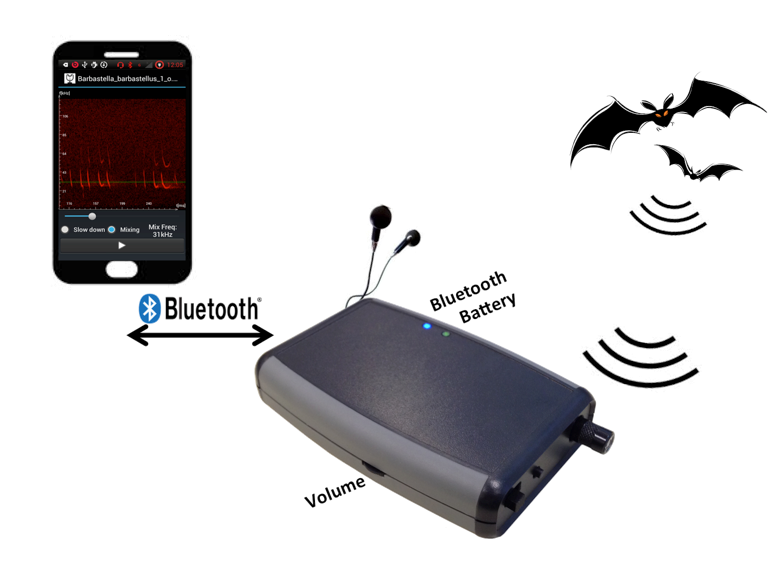
\includegraphics[height=60mm]{images/batcapture0.png}
        \graphicscaption{BatCapture im Einsatz}
    \end{minipage}%
    \begin{minipage}{0.5\textwidth}
        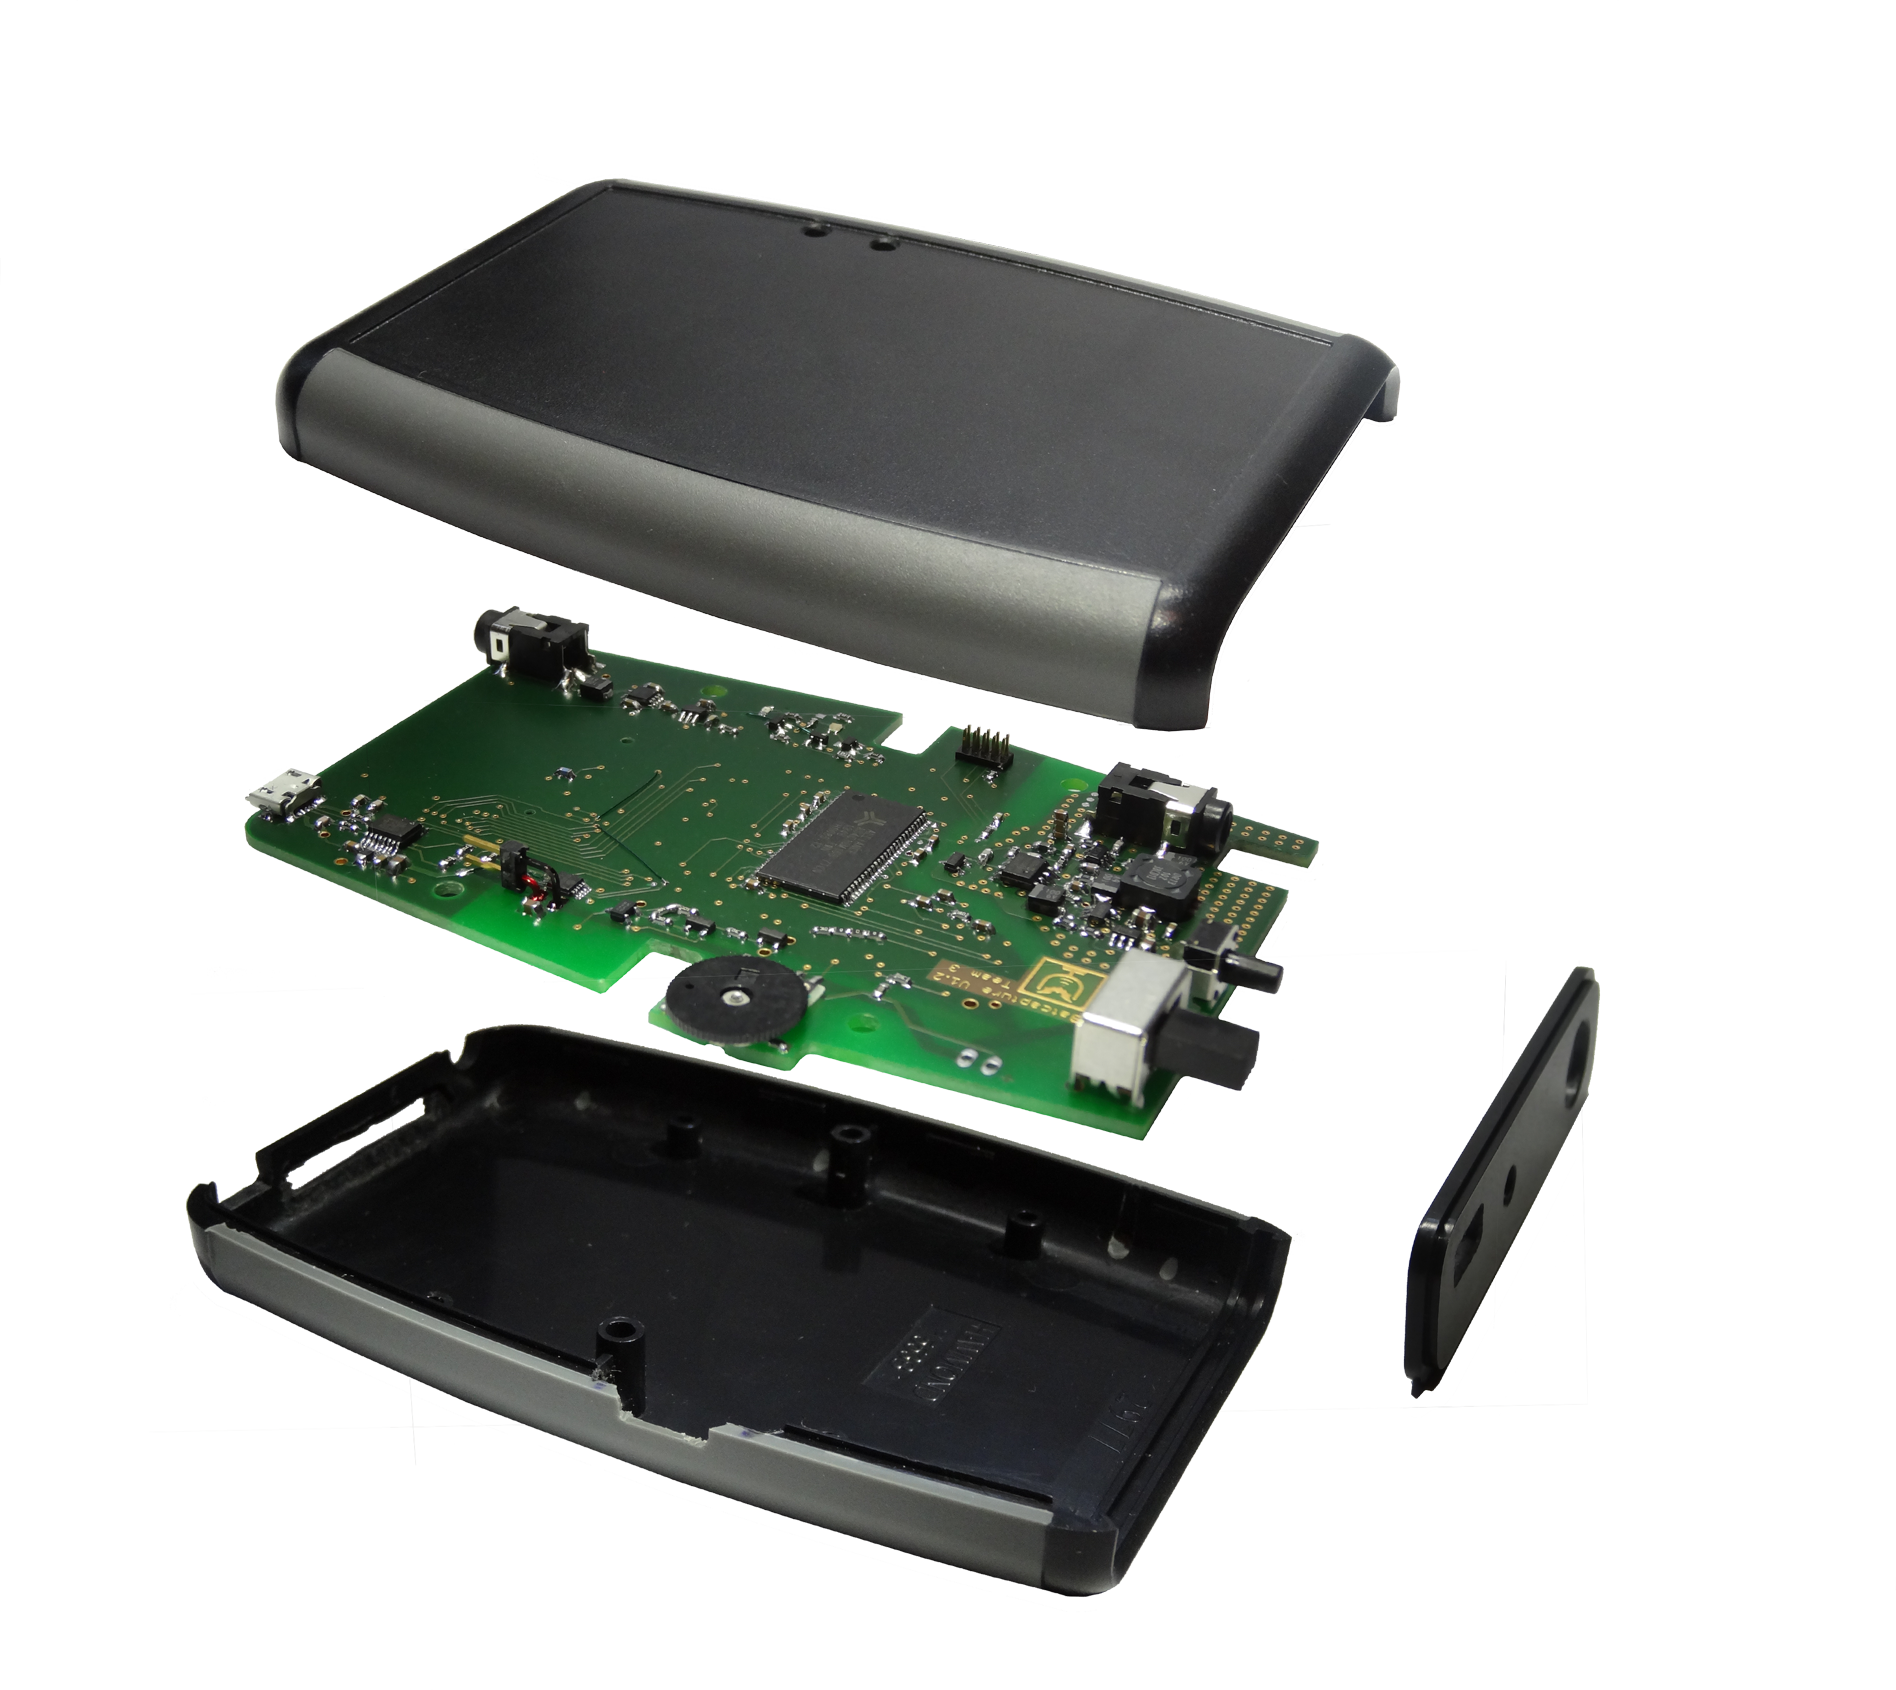
\includegraphics[height=60mm]{images/batcapture1.png}
        \graphicscaption{Zusammenstellung}
    \end{minipage}
    \graphicssource{Wikipedia}
}

\fscontent{
    \section{Die Aufgabe}
    Die meisten  Fledermausarten in  der Schweiz  sind bedroht. Um  sie besser
    schützen zu können, sollten so m\"oglichst viele Informationen über sie
    gesammelt werden.

    Für  die  Beobachtung von  Fledermäusen  werden bereits  verschiedene
    Geräte mit  Datenloggerfunktion auf dem Markt  angeboten. Warum also noch
    ein weiteres Produkt?

    Im  Gegensatz  zu existierenden  Produkten  auf  dem Logger,  erfolgt  die
    Auswertung  beim   BatCapture  auf  einem  Smartphone.    Damit  kann  der
    Datenlogger  auf  die   notwendigsten  Komponenten  reduziert  werden. Die
    Folgen:

    \emph{Ein handlicher,  energiesparsamer und  preiswerter Detektor  in noch
    nie dagewesener Form!}

    \section{Die L\"osung}
    
    Der  BatCapture  ist mit  einem  für  den Ultraschallbereich  optimierten
    Mikrofon  ausgerüstet.

    Das Herzstück der  Analyse besteht aus einer FFT  auf dem Mikrocontroller
    des  BatCapture. Fledermausrufe werden  von anderen  Quellen unterschieden
    und lokal abgespeichert.

    Via  Bluetooth werden  die  Daten an  das  Smartphone gesendet. Durch  das
    Spektrogramm  können  die  Rufe   analysiert  und  im  hörbaren  Bereich
    abgespielt  werden.

    \section{Die Bedienung}
    Nach Betätigung  des Schiebeschalters  kann durch den  Pairing-Taster der
    BatCapture  mit  der  App  automatisch  verbunden  werden.   Während  des
    Betriebs  zeigt eine  LED den  Status des  Akkus an,  der über  Micro-USB
    geladen werden kann.

    Die Mithörfunktion  wird mit anschliessbaren  Kopfhörern am BatCapture
    wahrgenommen. Die Lautstärke ist über ein Potentiometer regulierbar.

    Sämtliche aufgezeichneten Rufe können auf  dem Smartphone mit  Hilfe von
    Tags geordnet, abgespielt und nach Belieben grafisch analysiert werden.
}

\infobox{Highlights}{%
    \footnotesize
    \setlength\tabcolsep{2pt}
    \begin{tabular}{lp{25mm}lp{30mm}}
    \bfseries App    &                         & \bfseries BatCapture &                      \\
    Android-Version: & ab 4.0                  & Akkulaufzeit         & >\SI{10}{\hour}      \\
    Funktionen:      & Crest-Faktor            & Schnittstellen:      & Ein-/Ausschalter     \\
                     & Datei-Verwaltung        &                      & Micro-USB (Laden)    \\
                     & Bluetooth-Konfiguration &                      & Lautst\"arkeregelung \\
    Anzeige:         & Spektrogramm            &                      & \SI{3.5}{\mm} Klinke \\
    Kosten:          & keine                   &                      & SD-Karte (Specher)   \\
                     &                         & Versorgung:          & Akku Li-Io \SI{1880}{\milli\ampere\hour}, \SI{3.7}{\volt} \\
                     &                         & Speicher:            & \SI{256}{\mega\byte} \\
                     &                         & Verbingung:          & Bluetooth            \\
                     &                         & Abmessungen:         & $\num{117} \times \num{79} \times \SI{24}{\mm^3}$ \\
    \end{tabular}
}
